%%%%%%%%%%%%%%%%%%%%%%%%%%%%%%%%%%%%%%%%%%%%%%%%%%%%%%%%%%%%%%%%%%%%%%%%%%%%%%%%
% ISE Lab -- Topic
% Giovanni Ciatto
% Alma Mater Studiorum - Università di Bologna
% mailto:giovanni.ciatto@unibo.it
%%%%%%%%%%%%%%%%%%%%%%%%%%%%%%%%%%%%%%%%%%%%%%%%%%%%%%%%%%%%%%%%%%%%%%%%%%%%%%%%
%\documentclass[handout]{beamer}\mode<handout>{\usetheme{default}}
%
\documentclass[presentation]{beamer}\mode<presentation>{\usetheme{AMSBolognaFC}}
%\documentclass[handout]{beamer}\mode<handout>{\usetheme{AMSBolognaFC}}
%%%%%%%%%%%%%%%%%%%%%%%%%%%%%%%%%%%%%%%%%%%%%%%%%%%%%%%%%%%%%%%%%%%%%%%%%%%%%%%%
\usepackage{ise-lab-common}
\usepackage{ise-lab-ilp}
% version
\newcommand{\versionmajor}{0}
\newcommand{\versionminor}{1}
\newcommand{\versionpatch}{1}
\newcommand{\version}{\versionmajor.\versionminor.\versionpatch}
%%%%%%%%%%%%%%%%%%%%%%%%%%%%%%%%%%%%%%%%%%%%%%%%%%%%%%%%%%%%%%%%%%%%%%%%%%%%%%%%
\title[\currentLab{} -- Symbolic ML \& ILP]{
    Symbolic Machine Learning and Inductive Logic Programming
}
%
\subtitle{\courseName{} / Module \moduleN{} (\courseAcronym)}
%
\author[\sspeaker{\gcShort}]{\speaker{\gcFull} \\ \gcEmail}
%
\institute[\disiShort, \uniboShort]{\disi{} (\disiShort)\\\unibo}
%
\date[A.Y. \academicYear{} (v.\ \version)]{Academic Year \academicYear{}\\(version \version)}
%
%%%%%%%%%%%%%%%%%%%%%%%%%%%%%%%%%%%%%%%%%%%%%%%%%%%%%%%%%%%%%%%%%%%%%%%%%%%%%%%%
\begin{document}
%%%%%%%%%%%%%%%%%%%%%%%%%%%%%%%%%%%%%%%%%%%%%%%%%%%%%%%%%%%%%%%%%%%%%%%%%%%%%%%%

%/////////
\frame{\titlepage}
%/////////

%%===============================================================================
\section*{Outline}
%%===============================================================================
%
%%/////////
\frame[c]{\tableofcontents[hideallsubsections]}
%%/////////

%===============================================================================
\section{Machine Learning}
%===============================================================================

\begin{frame}[allowframebreaks]
\frametitle{Machine Learning (ML)}
    \begin{block}{A famous definition of ML from \cite{Mitchell1997}:}\itshape
        A computer program is said to learn from \alert{experience $E$} with respect to some class of \alert{tasks $T$} and \alert{performance $P$} if its performance at tasks in $T$, as measured by $P$, improves with experience $E$
    \end{block}

    \begin{alertblock}{Very \textbf{wide} definition, not specifying:}
        %
        \begin{itemize}
            \item what are the possible tasks?
            \item how performance is measured for a given task?
            \item what is experience?
            \item how / when experience should be provided to programs?
            \item what parts of the program are supposed to change via learning?
            \item under which form learnt information is represented?
        \end{itemize}
    \end{alertblock}
\end{frame}

\begin{frame}[allowframebreaks]
\frametitle{Many ways to categorise ML}
    \begin{block}{Supervised, unsupervised, reinforcement learning}
        \begin{itemize}
            \item \textbf{Supervised} learning:
            %
            \begin{itemize}
                \item[$T$] $=$ approximation for unknown \alert{relation}  
                \item[$E$] $=$ a statistically-relevant \alert{sample} of that relation
                \item[$P$] $=$ a \alert{quality measure} for the approximation
            \end{itemize}

            \item \textbf{Unsupervised} learning:
            %
            \begin{itemize}
                \item[$E$] $=$ \alert{set} of \alert{homogeneous} data 
                \item[$T$] $=$ \alert{partitioning} of data into multiple sets
                \item[$P$] $=$ \alert{optimality criterion} intensionally describing the partitioning 
            \end{itemize} 

            \item \textbf{Reinforcement} learning:
            %
            \begin{itemize}
                \item[$T$] $=$ letting agents choose actions in states  
                \item[$E$] $=$ \alert{reward} received for achieving a goal 
                \item[$P$] $=$ \alert{optimality criterion} for the policy
            \end{itemize} 
        \end{itemize}
    \end{block}

    \begin{block}{Symbolic vs. sub-symbolic learning}
        \begin{itemize}
            \item depends on whether the learnt information can be \alert{symbolically} represented or not
        \end{itemize}
    \end{block}

    \begin{block}{On-line vs. off-line learning}
        \begin{description}
            \item[Off-line] $\approx$ learning occurs \alert{before} operation
            \item[On-line] $\approx$ learning occurs \alert{during} operation
        \end{description}
    \end{block}
    
    \begin{center}
        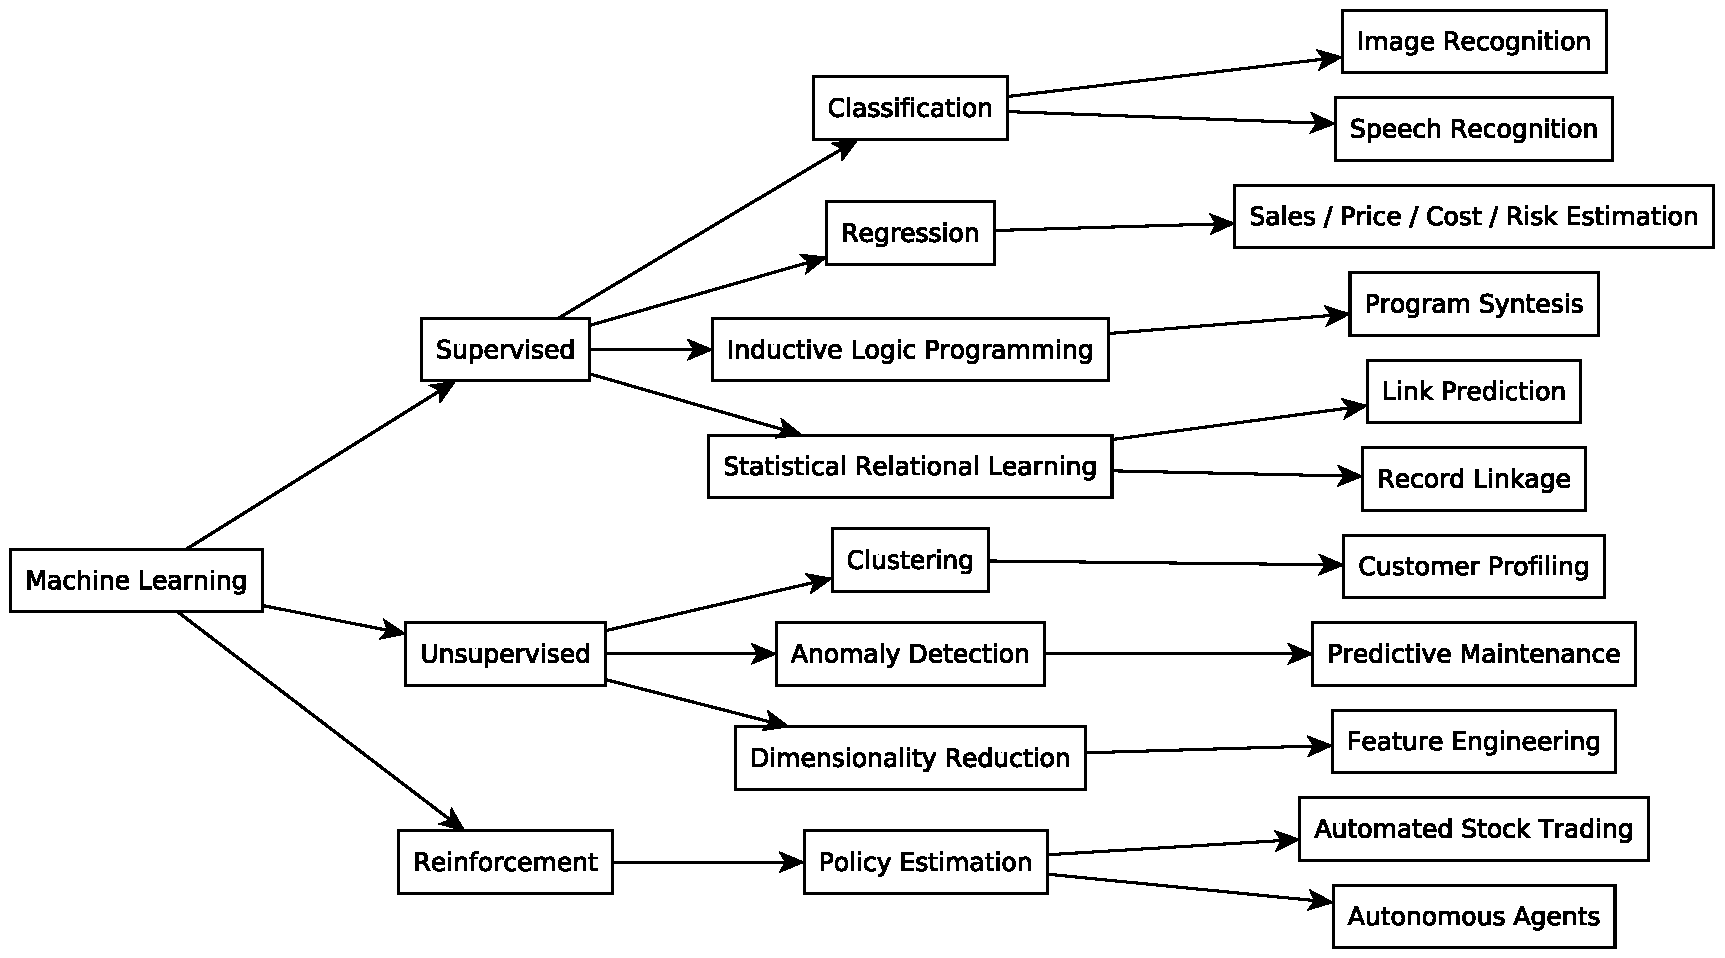
\includegraphics[width=.7\linewidth]{figures/ml-taxonomy.pdf}
    \end{center}
\end{frame}

%===============================================================================
\section{Symbolic Machine Learning}
%===============================================================================

\begin{frame}[allowframebreaks]
\frametitle{Symbolic Supervised Learning}

    \begin{block}{Insights}
        \begin{itemize}
            \item Aims at learning a \alert{relation from examples} (supervised)
            \item The learnt relation is a \alert{logic program} (symbolic)
            \item May learn \alert{intensional} representations too
            \item Two major (partially overlapping) branches:
            %
            \begin{itemize}
                \item inductive logic programming (ILP) \cite{Muggleton1991}
                \item statistical relational learning (SRL) \cite{DeRaedt2010,RaedtK04}
            \end{itemize}
        \end{itemize}
    \end{block}

    \begin{block}{Formulation \cite{DeRaedt2010}}
        Given
        %
        \begin{itemize}
            \item a \alert{background knowledge} $B$, i.e. a theory of known clauses
            \item a set of \alert{positive examples} $E^+$, i.e. a theory of ground, \alert{true} facts
            %
            % \begin{itemize}
            %     \item known to be 
            % \end{itemize}
            \item a set of \alert{negative examples} $E^-$, i.e. a theory of ground, \alert{false} facts
            %
            % \begin{itemize}
            %     \item known to be \alert{false}
            % \end{itemize}
        \end{itemize}
        %
        the goal is to 
        %
        \begin{itemize}
            \item \alert{(parameters learning)} tune a \alert{known} (yet \alert{parametric}) theory
            %
            \begin{itemize}
                \item possibly leveraging on clauses in $B$
                \item maximising the probability of $E^+$ being true
                \item minimising the probability of $E^-$ being false
            \end{itemize}
            %
            \item \alert{(structure learning)} induce a theory \alert{from scratch}
            %
            \begin{itemize}
                \item possibly leveraging on clauses in $B$
                \item from which all facts in $E^+$ and no facts in $E^-$ can be proved
            \end{itemize}
        \end{itemize}
    \end{block}

    \begin{block}{Learning as search}
        Both in structure and parameter learning
        %
        \begin{itemize}
            \item the goals is \alert{searching} for some \alert{optimal} theory $H^*$\ldots
            \item \ldots among a set of admissible hypotheses $\mathcal{H}$
            \item assumptions are commonly made on the admissible shapes all $H \in \mathcal{H}$
        \end{itemize}
    \end{block}
\end{frame}

\begin{frame}[allowframebreaks]
    \frametitle{Examples}

    Parameters learning:
    %
    \prologimport{listings/slr-example.pl}

    \begin{exampleblock}{Here the goal is tuning the \textbf{probabilities}}
        \begin{itemize}
            \item $\alert{p} = 75\%$, \qquad $\alert{q} = 25\%$
        \end{itemize}
    \end{exampleblock}

    \framebreak

    Structure learning:
    %
    \prologimport{listings/ilp-example.pl}
    %
    \begin{exampleblock}{Here the goal is \textbf{inducing} the theory}
        \begin{itemize}
            \item \prolog{grand_parent(X, Y) :- grand_parent(X, Z), grand_parent(Z, Y).}
        \end{itemize}
    \end{exampleblock}
\end{frame}

%===============================================================================
\section{Inductive Logic Programming}
%===============================================================================

\startExercise

\begin{frame}{\currentExercise{} -- First Exercise}
    \begin{block}{Goal}
        Goal here
    \end{block}
    %
    \begin{itemize}
        \item further info here
    \end{itemize}
\end{frame}

%===============================================================================
\section*{}
%===============================================================================

%/////////
\frame{\titlepage}
%/////////

%===============================================================================
\section*{\refname}
%===============================================================================

%%%%
\setbeamertemplate{page number in head/foot}{}
%/////////
% \begin{frame}[c,noframenumbering]{\refname}
\begin{frame}[t,allowframebreaks,noframenumbering]{\refname}
%	\tiny
    \scriptsize
%	\footnotesize
    \nocite{*}
    \bibliographystyle{apalike-AMS}
    \bibliography{ise-lab-ilp}
\end{frame}
%/////////

%%%%%%%%%%%%%%%%%%%%%%%%%%%%%%%%%%%%%%%%%%%%%%%%%%%%%%%%%%%%%%%%%%%%%%%%%%%%%%%%
\end{document}
%%%%%%%%%%%%%%%%%%%%%%%%%%%%%%%%%%%%%%%%%%%%%%%%%%%%%%%%%%%%%%%%%%%%%%%%%%%%%%%%
